\documentclass[11pt]{article}
\usepackage[a4paper,includeheadfoot,margin=2.54cm]{geometry}
\usepackage{parskip}

% fonte adotada
\usepackage{mathpazo}
\usepackage{domitian}
\usepackage[T1]{fontenc}
\let\oldstylenums\oldstyle

\usepackage{hyperref}
\usepackage{graphicx}

\begin{document}

\underline{\textbf{Atividade 15 - Diagrama de Loop Casual}}\par
\textbf{Sistemas de Informação}\\
\textbf{Instituto Federal do Espírito Santo}\\
Campus Serra - Espírito Santo\par
\textbf{Teoria Geral de Sistemas}\\
Prof. Dr. Rodrigo Fernandes Calhau\par
Anderson A. Fraga (20222BSI0482)\\
\texttt{aafrg@tuta.io}\\  %\texttt formats the text to a typewriter style font

\begin{enumerate}
	\item Realizar o diagrama de loop causal (mapa sistêmico) relativo ao estudo de caso 2 na página 184 do livro \href{https://drive.google.com/file/d/1eJU2qK8IzC-S8jRKQuHrIgED1tEvzGOq/view}{Desvendando Sistemas}.

		\textbf{1o ciclo - a ação dos oceanos}\par
		\begin{figure}[!h]
			\centering
			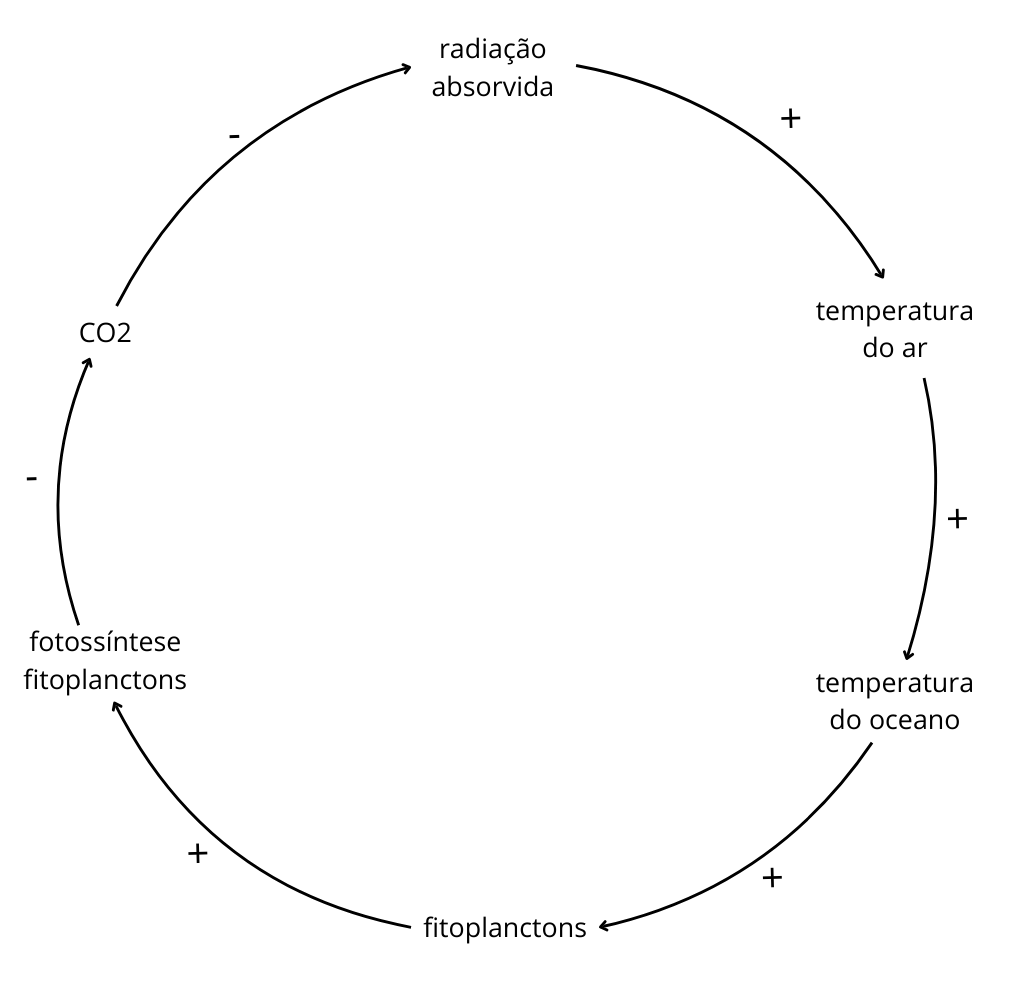
\includegraphics[width=0.75\linewidth]{mapa1-1.png}
		\end{figure}
\pagebreak
        \textbf{2o ciclo - a ação das florestas}\par
		\begin{figure}[!ht]
			\centering
			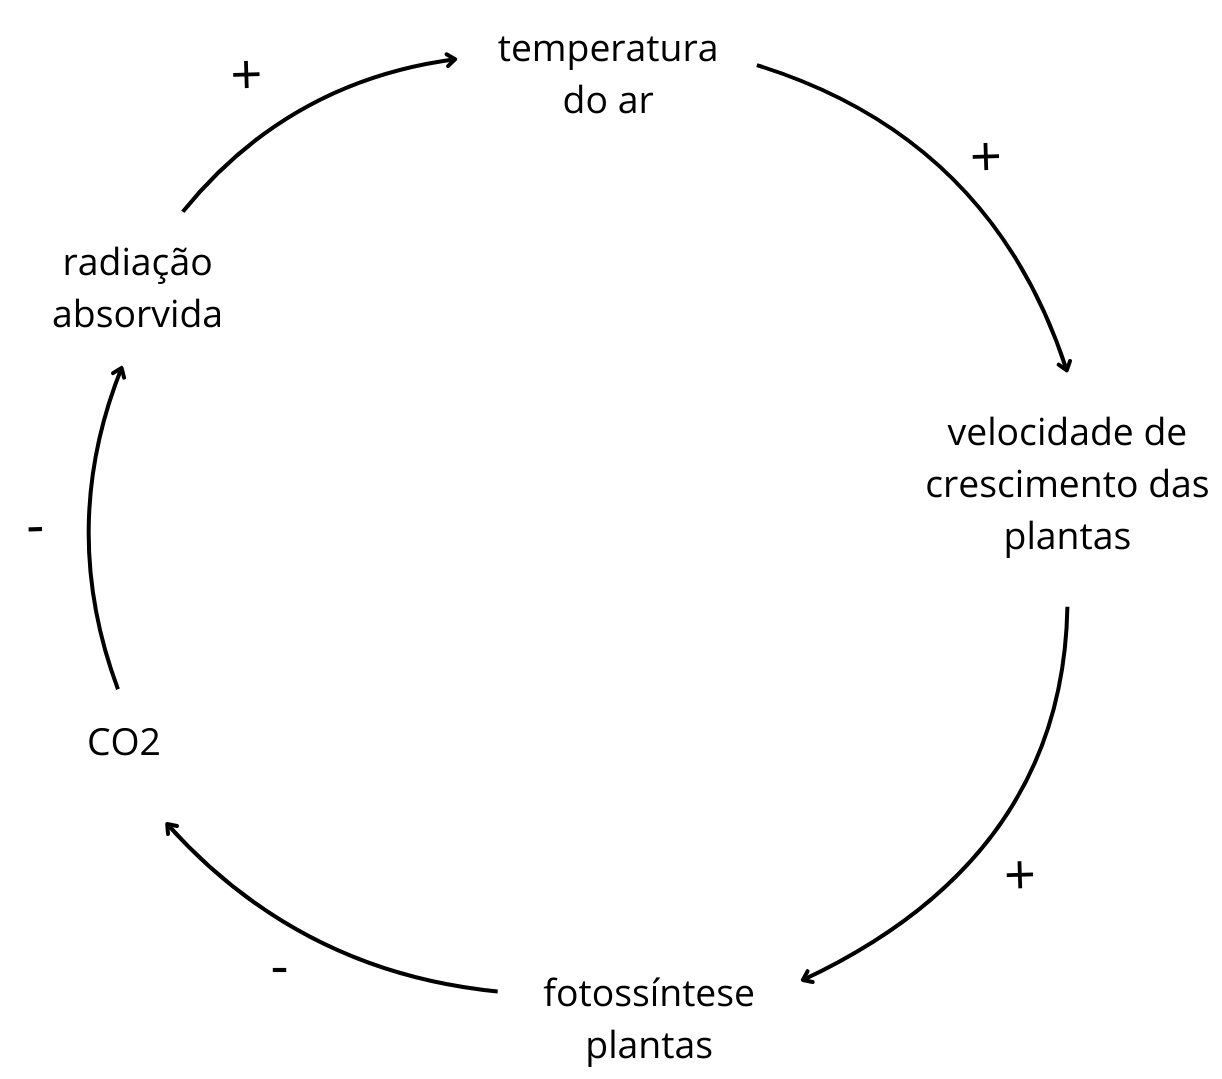
\includegraphics[width=0.75\linewidth]{mapa1-2.png}
		\end{figure}

        \textbf{3o ciclo - a ação das calotas polares}\par
		\begin{figure}[!ht]
			\centering
			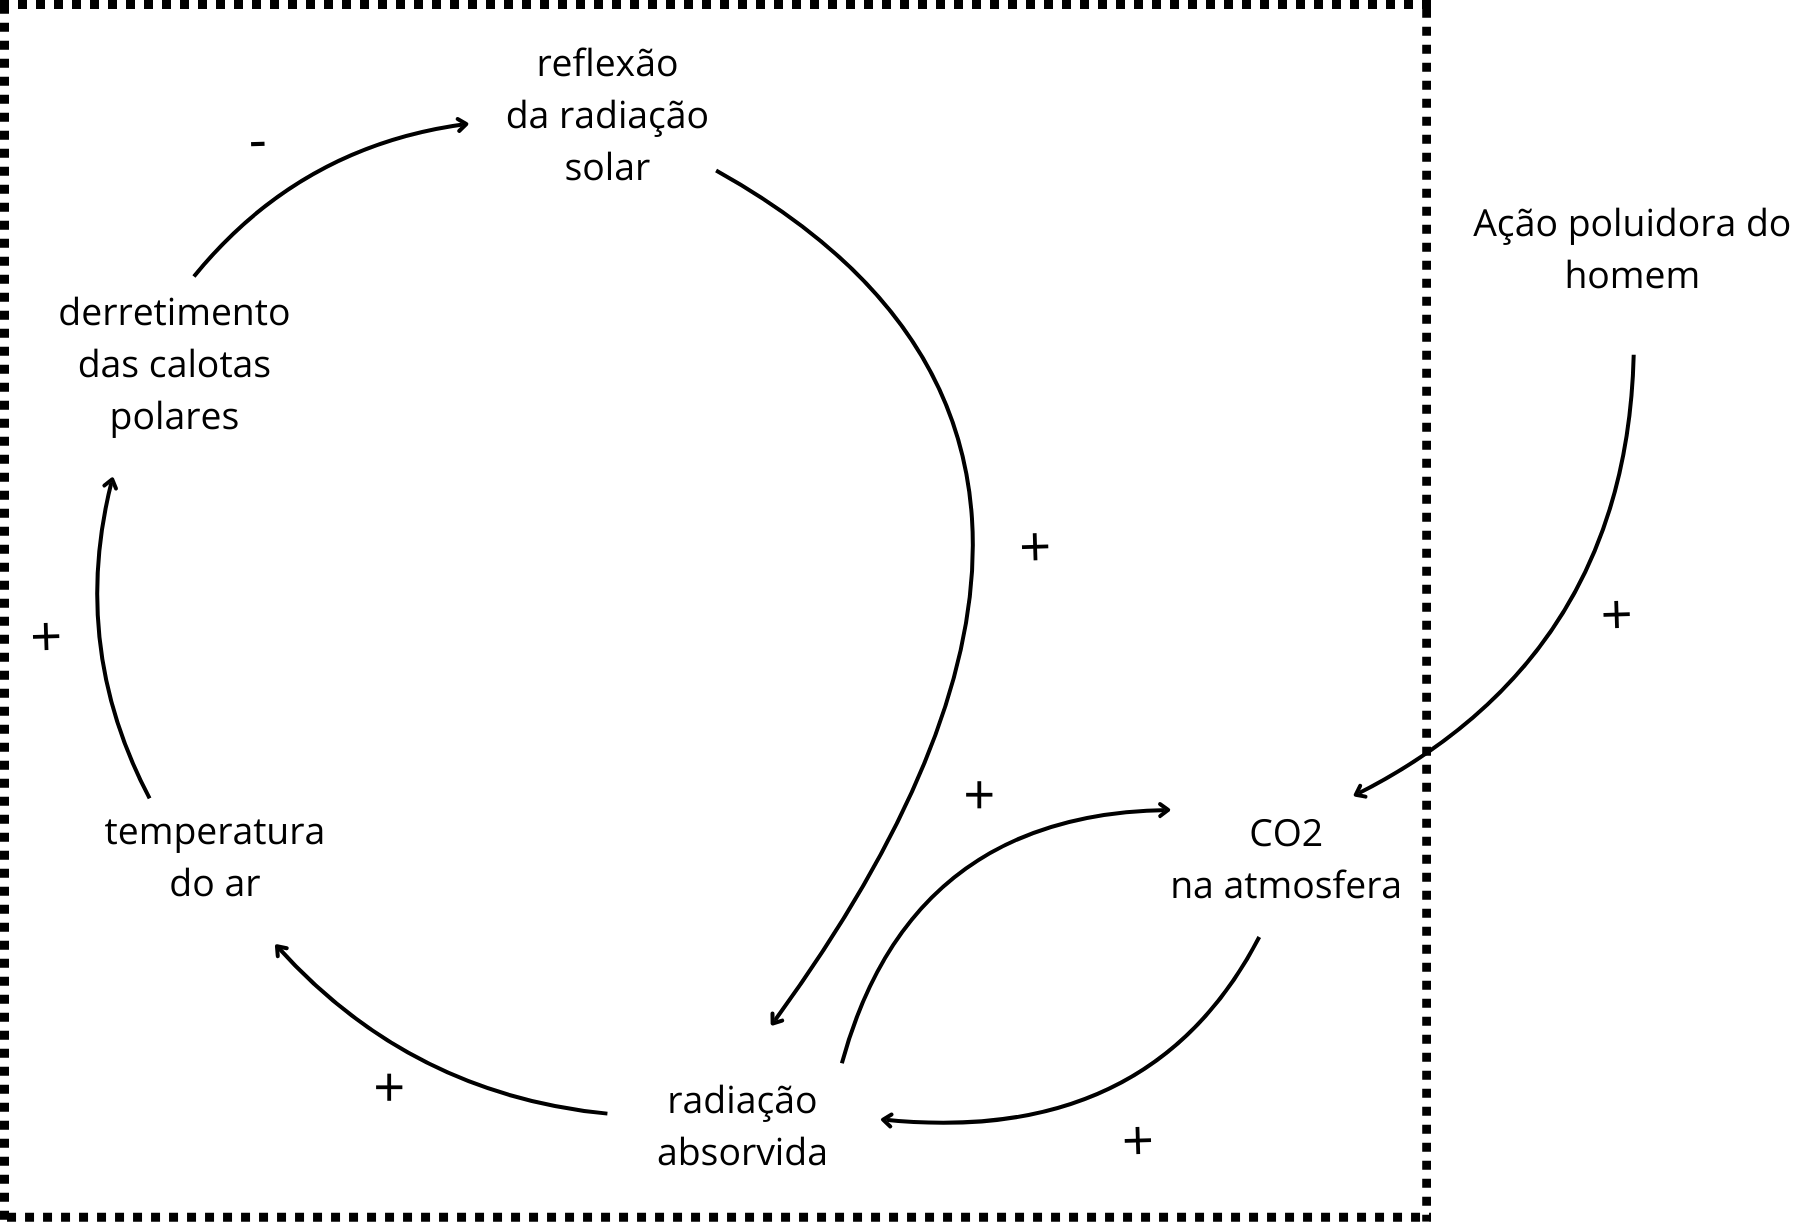
\includegraphics[width=0.79\linewidth]{mapa1-3.png}
		\end{figure}
\pagebreak
        \textbf{4o ciclo - a ação do permafrost}\par
		\begin{figure}[!ht]
			\centering
			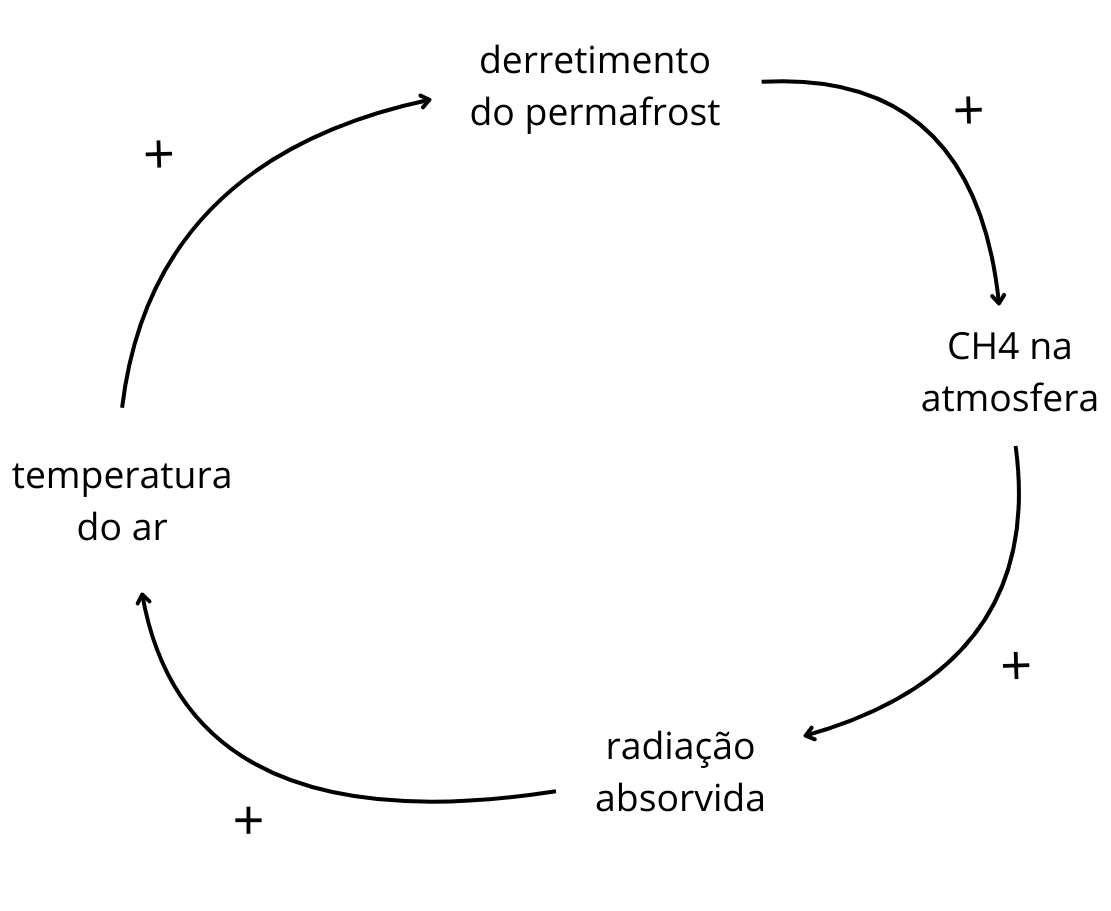
\includegraphics[width=0.79\linewidth]{mapa1-4.png}
		\end{figure}

    \item Realizar o diagrama de loop causal (mapa sistêmico) relativo ao estudo de caso 3 na página 186 do livro \href{https://drive.google.com/file/d/1eJU2qK8IzC-S8jRKQuHrIgED1tEvzGOq/view}{Desvendando Sistemas}.
        %\textbf{Análise de estratégias governamentais}\par
		\begin{figure}[!ht]
			\centering
			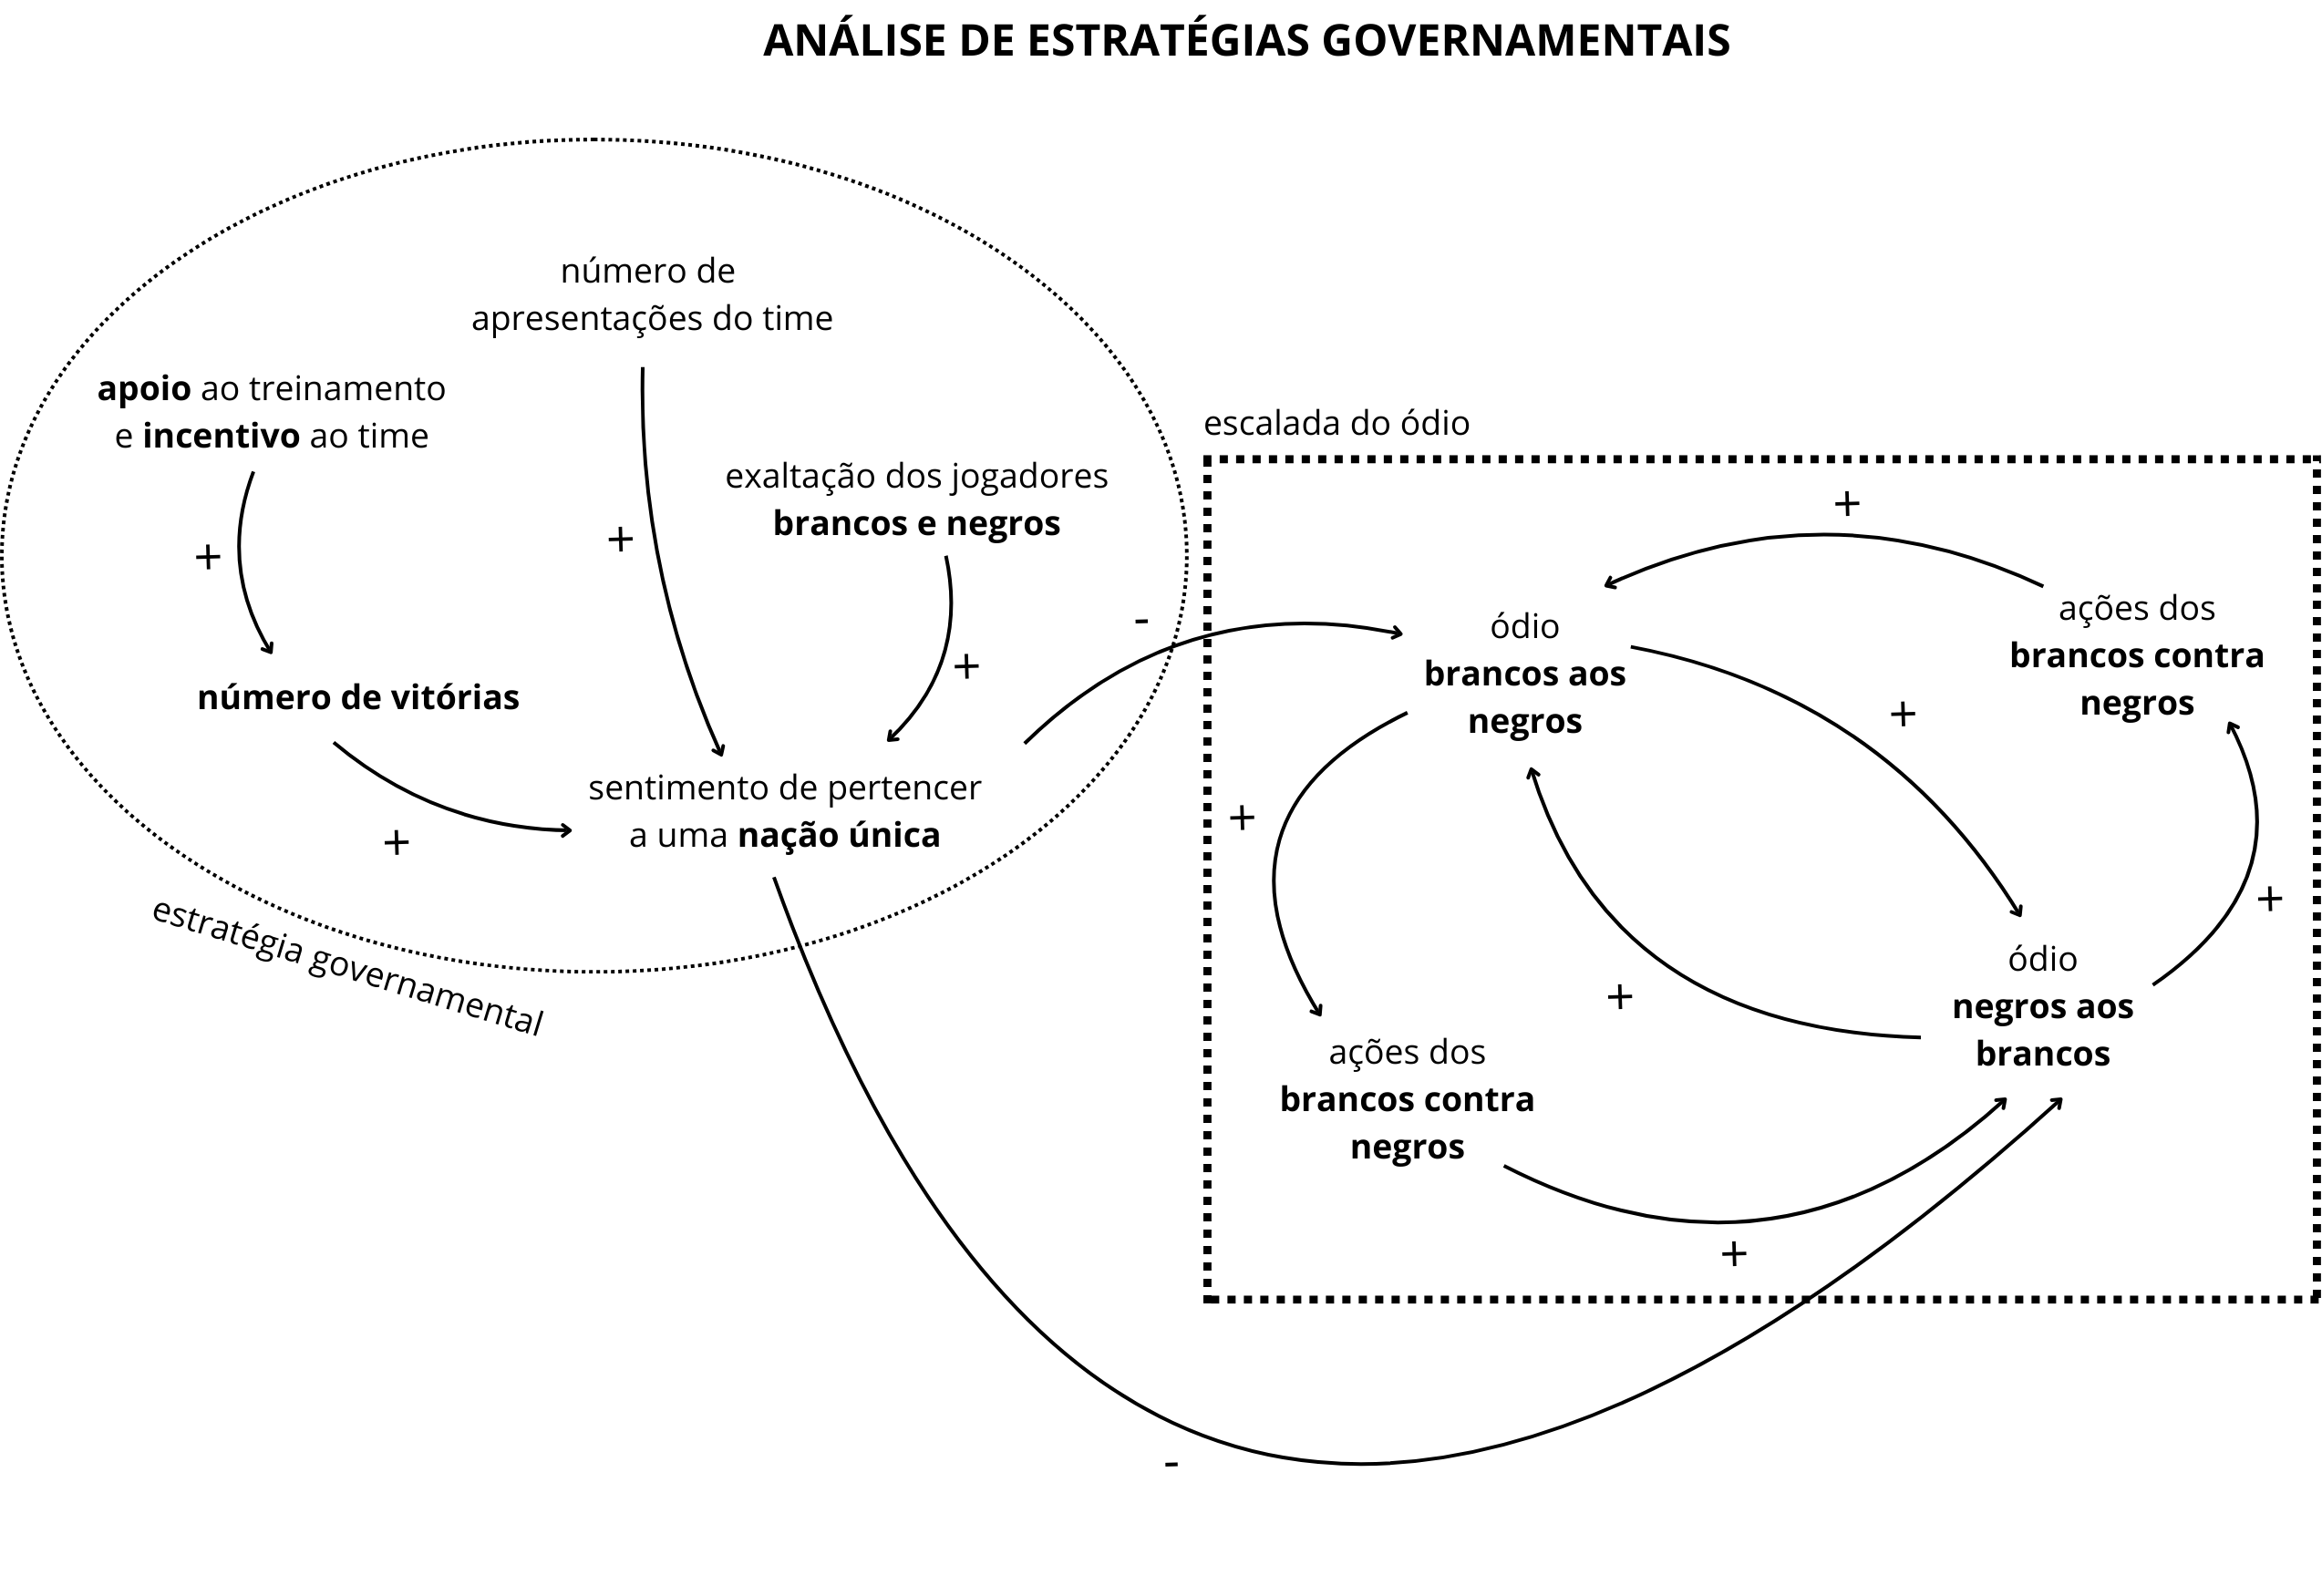
\includegraphics[width=0.83\linewidth]{mapa2-1.png}
		\end{figure}

\end{enumerate}

\end{document}
